\section{S6 -- Metody komunikacji międzyprocesowej w systemach lokalnych i rozproszonych}

\textbf{Komunikacja międzyprocesowa} -- (\textit{Inter-Process Communication} -- IPC) -- sposób komunikacji pomiędzy wieloma procesami systemu operacyjnego uruchomionego na maszynie lokalnej, bądź rozproszonej grupie autonomicznych maszyn połączonych w sieć. Techniki komunikacji możemy podzielić na:
\begin{itemize}
	\item Przekazywanie komunikatów
    \item Synchronizację
    \item Współdzielenie pamięci
    \item Wywoływanie procedur
\end{itemize}

Główne cechy systemu rozproszonego:
\begin{itemize}
	\item \textbf{Dzielenie zasobów} -- maszyny rozproszonego systemu mają możliwość współdzielenia urządzeń (np. drukarki, skanery), dzielenia plików oraz usług
    \item \textbf{Otwartość} -- podatność na rozszerzenia, możliwość rozbudowy systemu zarówno sprzętowo jak i programowo
    \item \textbf{Współbieżność} -- zdolność przetwarzania wielu zadań równocześnie
    \item \textbf{Skalowalność} -- zachowanie podobnej wydajności systemu przy zmienianiu skali systemu (np. dodawanie nowych maszyn, procesorów)
    \item \textbf{Tolerowanie awarii} -- zdolność do dalszego działania systemu mimo wystąpienia błędów w oprogramowaniu lub uszkodzeń fizycznych
    \item \textbf{Przezroczystość} -- cały system zachowuje się tak, jakbyśmy pracowali na jednej maszynie, nie zaś na wielu osobnych jednostkach połączonych w jeden system
\end{itemize}

\begin{table}[!ht]
\centering
\caption{Metody komunikacji międzyprocesowej}
\label{ipc}
\begin{tabular}{|l|l|c|c|}
\hline
\multicolumn{1}{|c|}{\textbf{Metoda komunikacji}} & \multicolumn{1}{c|}{\textbf{Systemy operacyjne}} & \textbf{Lokalne} & \textbf{Rozproszone} \\ \hline
Pliki & Większość systemów & tak & tak \\ \hline
Gniazdka & Większość systemów & tak & tak \\ \hline
Sygnały & POSIX & tak & nie \\ \hline
Kolejki komunikatów & POSIX, Windows & tak & nie \\ \hline
Łącza nienazwane & POSIX, Windows & tak & nie \\ \hline
Łacza nazwane & POSIX, Windows & tak & nie \\ \hline
Semafory & POSIX, Windows & tak & nie \\ \hline
Pamięć współdzielona & POSIX, Windows & tak & nie \\ \hline
Zmapowany plik & POSIX, Windows & tak & tak \\ \hline
\begin{tabular}[c]{@{}l@{}}Przekazywanie\\ komunikatów\end{tabular} & \begin{tabular}[c]{@{}l@{}}Systemy z MPI, RPC,\\ COBRA, Java RMI\end{tabular} & tak & tak \\ \hline
\end{tabular}
\end{table}

\subsection{Pliki}

Jest to najłatwiejszy sposób wymagający jedynie otwarcia pliku. Dla zachowania spójności danych tylko jeden proces może zapisywać do pliku w danym czasie, zaś czytać może nieograniczona ilość procesów. Występuje tutaj potrzeba zastosowania jakiegoś sposobu synchronizacji procesów zapisujących i informowania innych o zmianach. Komunikacja może odbywać się w obrębie jednego systemu operacyjnego, bądź też między różnymi systemami współdzielącymi przestrzeń dyskową.

Przykłady funkcji POSIX:
\begin{itemize}
	\item \texttt{fopen()} -- otwarcie pliku
    \item \texttt{fwrite()} -- zapis do pliku
    \item \texttt{fread()} -- odczyt z pliku
    \item \texttt{fclose()} -- zamknięcie pliku
\end{itemize}

\subsection{Gniazdka}

Umożliwiają komunikację dwukierunkową w systemach lokalnych i rozproszonych -- pozwalają na odbieranie i wysyłanie danych po obu stronach. W systemach UNIX gniazdko traktowane jest jak deskryptor otwartego pliku, więc można na nim używać funkcji jak do plików (\texttt{read()}, \texttt{write()}, \texttt{close()}). Oba punkty końcowe połączenia identyfikowane są za pomocą adresu IP oraz portu. Komunikacja przebiegać może bezpołączeniowo po protokole UDP za pomocą ciągu niezależnych pakietów (datagramów), bądź połączeniowo po TCP czyli przy pomocy strumienia danych.

Przykłady funkcji POSIX:
\begin{itemize}
	\item \texttt{socket()} -- utworzenie gniazdka
    \item \texttt{bind()} -- nadanie gniazdku adresu
    \item \texttt{connect()} -- połączenie się z serwerem TCP
    \item \texttt{accept()} -- połączenie się z klientem TCP
    \item \texttt{listen()} -- rejestracja gniazdka TCP
    \item \texttt{send()}, \texttt{recv()} -- wysłanie i odebranie wiadomości TCP
    \item \texttt{sendto()}, \texttt{recvfrom()} -- wysłanie i odebranie wiadomości UDP 
    \item \texttt{write()}, \texttt{read()} -- wysłanie i odebranie wiadomości TCP a także UDP po wykonaniu asocjacji gniazdka funkcją \texttt{connect()}
    \item \texttt{close()} -- zamknięcie gniazdka
\end{itemize}

\subsection{Sygnały}

Znane także jako przerwania programowe -- są to asynchroniczne powiadomienia wysyłane do innych procesów wymagające natychmiastowej reakcji ze strony procesu. Źródłem przerwań może być system operacyjny gdy nastąpi wydarzenie awaryjne, wykonanie odpowiednich funkcji w programie, bądź zabicie programu spod konsoli funkcją kill. Po otrzymaniu przerwania, system zaprzestaje wykonywania aktualnych instrukcji (przerwana może być każda nie-atomowa operacja) i rozpoczyna obsługę przerwania wykonując ustalone wcześniej funkcje przechwyconych przerwań, bądź domyślne funkcje obsługi przerwań. Przechwycony może być każdy sygnał z wyjątkiem SIGKILL oraz SIGSTOP. Sygnały obsługiwane sątylko przy przejściu między trybem jądra systemu a trybem użytkownika.

\begin{figure}[!h]
\centering
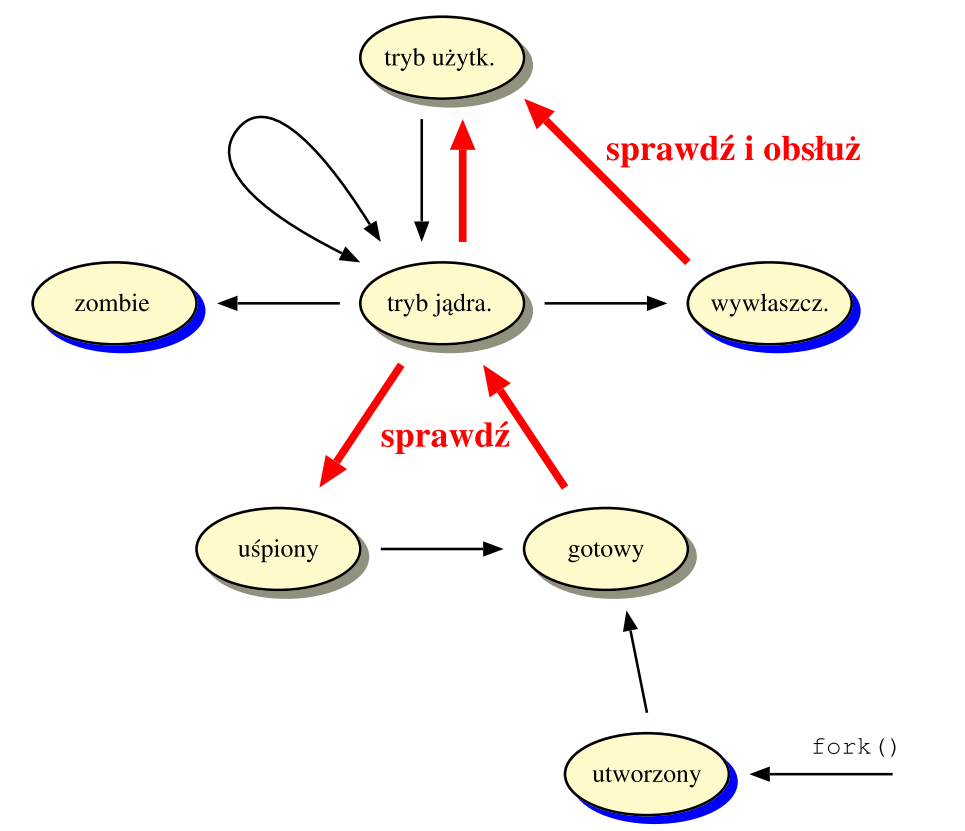
\includegraphics[width=0.6\textwidth]{s6_int_sygnaly.png}
\caption{Sygnały}
\end{figure}

Przykłady funkcji POSIX:
\begin{itemize}
	\item \texttt{signal()}, \texttt{sigset()} -- rejestruje funkcję obsługi sygnału
    \item \texttt{kill()}, \texttt{alarm()}, \texttt{raise()} -- wysyła sygnał
\end{itemize}

\subsection{Łącza nienazwane}

Jedna z prostszych metod komunikacji. Są to strumienie (pipe) pozwalające łączyć spokrewnione ze sobą procesy w relacji jednokierunkowej macierzysty -- potomny. Zazwyczaj są wykorzystywane do łączenia wyjścia stdout jednego procesu z wejściem stdin drugiego. Tworzenie łącza wypełnia dwuelementową tablicę deskryptorów, z czego pierwszy z nich jest końcem otwartym do czytania, a drugi służy do pisania. Oba końce traktowane są w systemie UNIX jako zwykłe deskryptory plików, więc można na nich używać funkcji jak do plików (\texttt{read()}, \texttt{write()}, \texttt{close()}). Nieużywany deskryptor musi zostać zamknięty funkcją \texttt{close()}. Jądro systemu gwarantuje, że operacje zapisu nie przekraczające rozmiaru bufora (w wielkości 4kB) są atomowe, niepodzielne. W powłokach systemów UNIX można używać łącza w formie pionowej linii do przesyłania wyników jednego polecenia do wejścia kolejnego.

\newpage

\begin{figure}[!h]
\centering
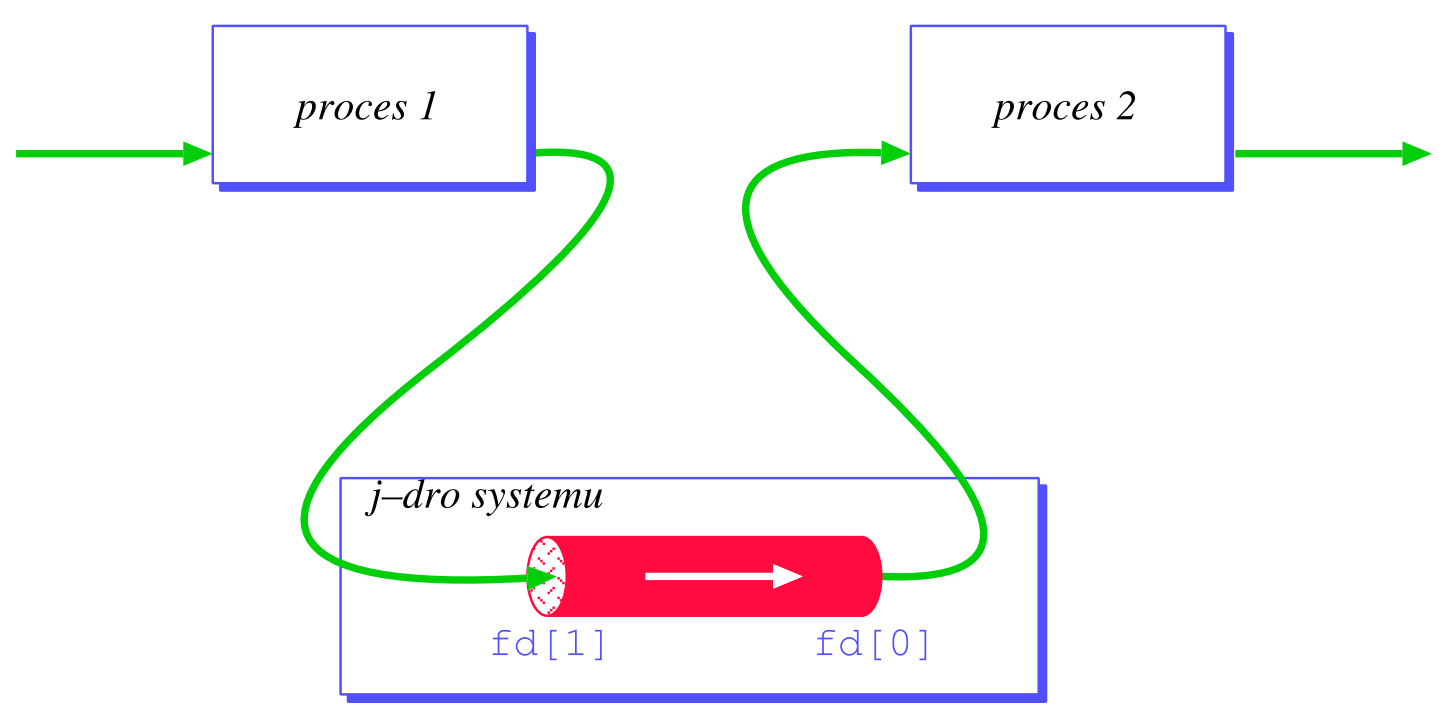
\includegraphics[width=0.8\textwidth]{s6_int_pipe.png}
\caption{Łącze nienazwane}
\end{figure}

Przykłady funkcji POSIX:
\begin{itemize}
	\item \texttt{pipe()} -- tworzy łącze nienazwane
    \item \texttt{dup()}, \texttt{dup2()} -- duplikowanie deskryptorów stdin, stdout
    \item \texttt{write()} -- zapisuje do łącza
    \item \texttt{read()} -- odczytuje z łącza
    \item \texttt{close()} -- zamyka łącze
\end{itemize}

\subsection{Łącza nazwane}

Inaczej strumienie FIFO, mogą być używane przez procesy w żaden sposób ze sobą nie spokrewnione, a nawet przez procesy różnych użytkowników. Szczególnie stosowane, gdy nie można zastosować relacji macierzysty -- potomny. Strumienie FIFO posiadają dowiązanie w systemie plików jako pliki specjalne -- oprócz atrybutów zwykłych plików takich jak nazwa, właściciel, grupa czy prawa dostępu, posiadają cechę dodatkową -- element odczytany z pliku FIFO jest z niego automatycznie usuwany. Funkcja użyta do otwarcia łącza blokuje proces do momentu otwarcia drugiego powiązanego łącza. Kolejki FIFO mają z reguły większy rozmiar 4-16kB.

Przykłady funkcji POSIX:
\begin{itemize}
	\item \texttt{mknod()} -- tworzy łącze nazwane
    \item \texttt{open()} -- otwiera łącze do pisania lub czytania
    \item \texttt{write()} -- zapisuje do łącza
    \item \texttt{read()} -- odczytuje z łącza
    \item \texttt{unlink()} -- usuwa łącze
\end{itemize}

\newpage

Miedzy łączami nienazwanymi a nazwanymi istnieje wiele podobieństw:
\begin{itemize}
	\item Zamknięcie końca do pisania generuje u czytelników EOF
    \item Zamknięcie końca do czytania generuje sygnał SIGPIPE u pisarzy
    \item Zapis i odczyt przez standardowe funkcje \texttt{read()} i \texttt{write()}
    \item Niepodzielność zapisu danych mniejszych niż rozmiar strumienia
    \item Blokowanie procesów w przypadku przepełnienia lub pustego bufora
\end{itemize}

\subsection{Kolejki komunikatów}

Jest to lista o określonej pojemności zawierająca komunikaty o zadanym maksymalnym rozmiarze. Komunikacja odbywa się tylko w jedną stronę -- nowe komunikaty dodawane są na koniec listy. Dzięki temu zachowana jest kolejność komunikatów. Każdy komunikat ma swój typ, dzięki czemu można obsługiwać kilka strumieni komunikatów w ramach jednej kolejki poprzez selektywne odbieranie komunikatów wybranego typu. Komunikacja odbywa się asynchronicznie, co znaczy, że odbiorca i nadawca nie muszą się łączyć w tym samym czasie. Komunikaty w kolejce ponadto przechowywane są do czasu odebrania ich przez inny proces. Kolejki komunikatów posiadają również inne ważne cechy:
\begin{itemize}
	\item Posiadają unikalne nazwy umożliwiające procesom identyfikację kolejki
    \item Można nadawać priorytety -- komunikaty o wyższym priorytecie są umieszczane na początku
    \item Wiele procesów może pisać i czytać do/z kolejki
    \item W kolejce mogą się znajdować komunikaty różnej długości (w przeciwieństwie do FIFO)
    \item Kolejce można przypisać maksymalną liczbę komunikatów -- po jej przekroczeniu, proces piszący zostaje zablokowany
    \item Można testować status kolejki, np. liczbę komunikatów (kolejki FIFO tego nie umożliwiają)
\end{itemize}

Przykłady funkcji POSIX:
\begin{itemize}
	\item \texttt{msgget()} -- tworzy kolejkę
    \item \texttt{msgsnd()} -- wysyła komunikat
    \item \texttt{msgrcv()} -- odbiera komunikat
    \item \texttt{msgctl()} -- modyfikuje parametry kolejki (usunięcie poprzez ustawienie parametru IPC\_RMID)
\end{itemize}

Przykłady funkcji System V:
\begin{itemize}
	\item \texttt{mq\_open()} - tworzy kolejkę
    \item \texttt{mq\_send()} - wysyła komunikat
    \item \texttt{mq\_receive()} - odbiera komunikat
    \item \texttt{mq\_close()} - zamyka kolejkę
    \item \texttt{mq\_unlink()} - usuwa kolejkę
\end{itemize}

\begin{figure}[!h]
\centering
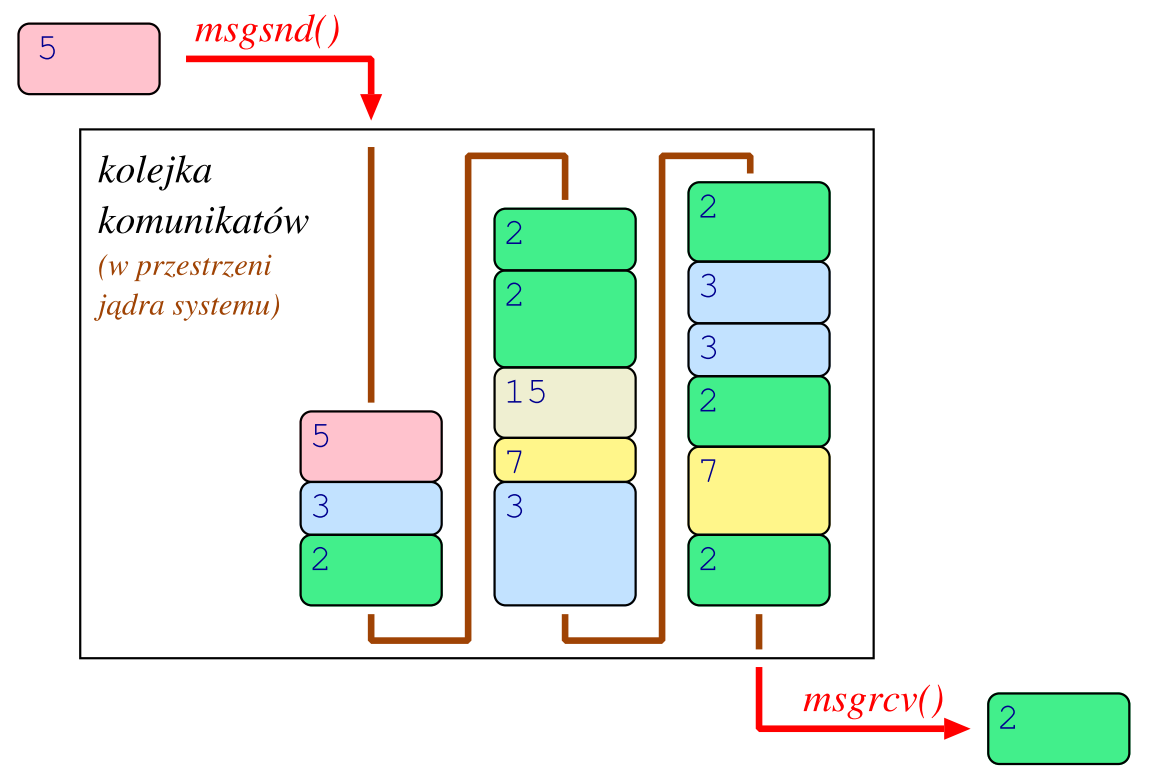
\includegraphics[width=0.8\textwidth]{s6_int_kolejka.png}
\caption{Kolejka komunikatów}
\end{figure}

\subsection{Funkcja select}

\subsection{Semafory}

chroniona zmienna systemowa, operacje atomowe V (inc), P (dec), nie może być < 0, synchronizacja procesów

\subsection{Pamięć współdzielona}

jeden proces tworzy obszar pamięci RAM, pozostałe mają do niego dostęp -- wspólny segment pamięci, odwzorowana jako własny obszar pamięci logicznej, wymaga dodatkowej synchronizacji

\subsection{Zmapowany plik w pamięci}

\subsection{Przekazywanie komunikatów}

RPC -- zdalne wywoływanie procedur
RMI -- technologia Java, stub
COBRA -- komunikacja między różnymi językami
MPI -- obliczenia wielowątkowe